\documentclass[tikz, border=1mm]{standalone}

\usepackage{pgfplots}
\pgfplotsset{compat=1.15}
\usepackage{mathrsfs}
\usetikzlibrary{arrows}
\pagestyle{empty}

\usepackage{amsmath,mathrsfs}

\usetikzlibrary{matrix,positioning,fit}
\newcommand{\mydot}{\raisebox{3ex}{$\cdots$}}

\begin{document}

\begin{tikzpicture}

\matrix (m)[matrix of math nodes,left delimiter=(,right delimiter=)]
{
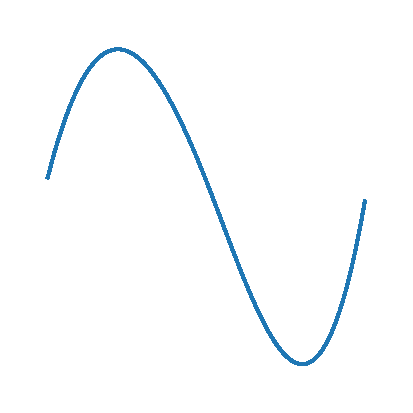
\includegraphics[scale=0.2]{for_data_matrix/1D-0.eps} & 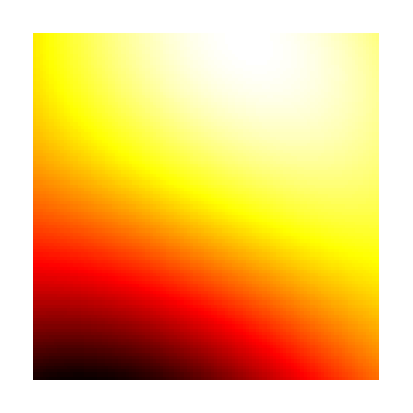
\includegraphics[scale=0.2]{for_data_matrix/2D-0.eps} & \mydot & 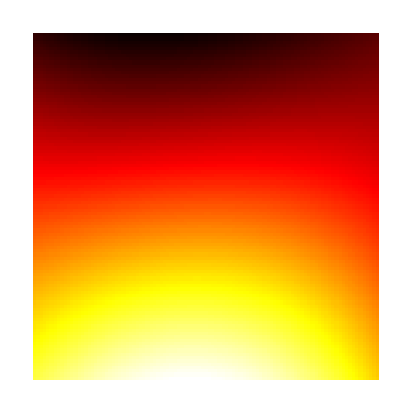
\includegraphics[scale=0.2]{for_data_matrix/2D-3.eps} & \mydot & 
\includegraphics[scale=0.2]{for_data_matrix/1D-3.eps} \\
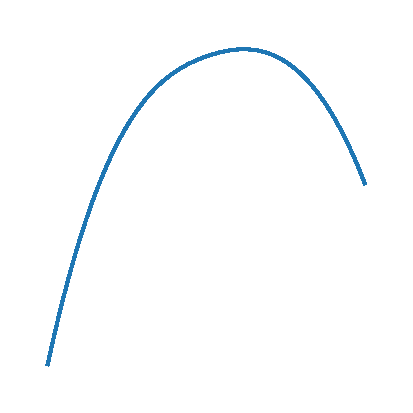
\includegraphics[scale=0.2]{for_data_matrix/1D-5.eps} & 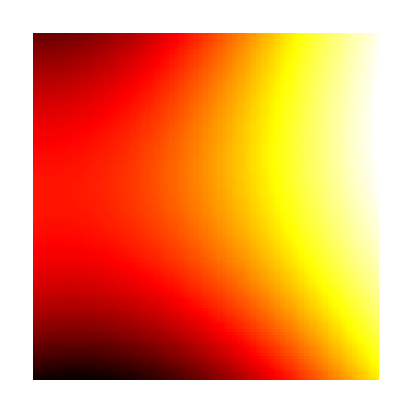
\includegraphics[scale=0.2]{for_data_matrix/2D-5.eps} & \mydot & 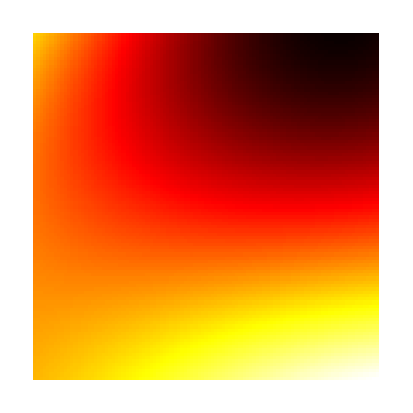
\includegraphics[scale=0.2]{for_data_matrix/2D-9.eps} & \mydot & 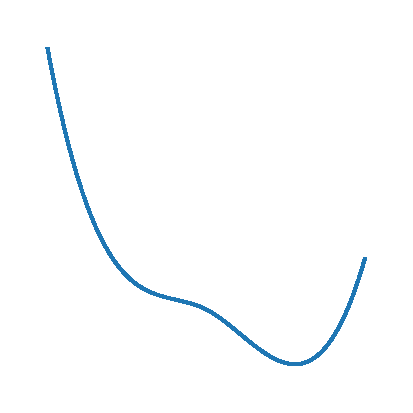
\includegraphics[scale=0.2]{for_data_matrix/1D-9.eps} \\
\vdots & \vdots      &       & \vdots &       & \vdots \\
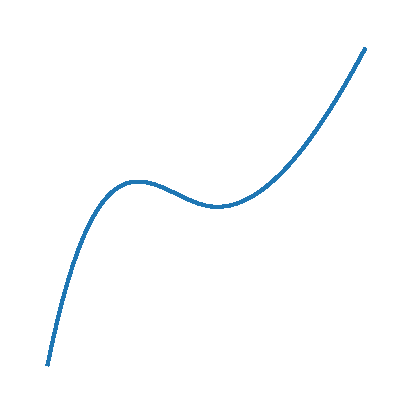
\includegraphics[scale=0.2]{for_data_matrix/1D-17.eps} & 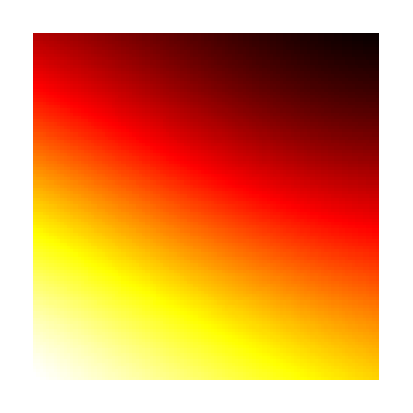
\includegraphics[scale=0.2]{for_data_matrix/2D-17.eps} & \mydot & 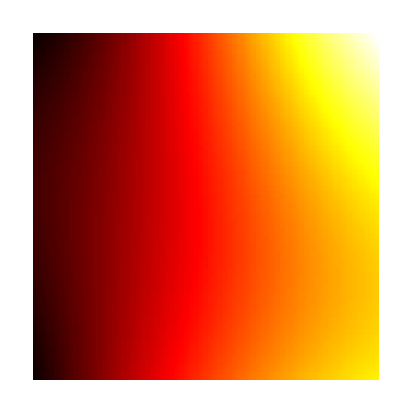
\includegraphics[scale=0.2]{for_data_matrix/2D-21.eps} & \mydot & 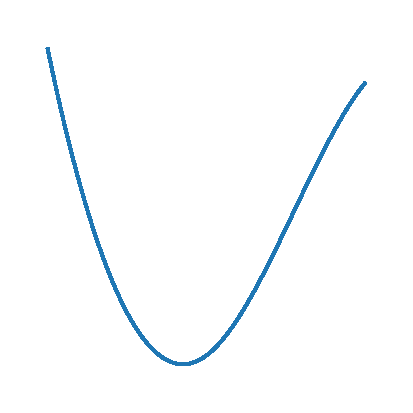
\includegraphics[scale=0.2]{for_data_matrix/1D-21.eps} \\
};

\end{tikzpicture}

\end{document}